\documentclass[smaller, aspectratio=169]{beamer}

% Packages

% -------------------------------
% Outer Theme Configuration
\useoutertheme{infolines} 

% -------------------------------
% Package Imports
% -------------------------------
\usepackage[utf8]{inputenc}        % UTF-8 encoding
\usepackage[english]{babel}        % English language support
\usepackage{amsmath}               % For math symbols and environments
\usepackage{amssymb}               % For additional math symbols
\usepackage{amsfonts}              % For math fonts
\usepackage{amsthm}                % For theorem environments
\usepackage{graphicx}              % For including graphics
\usepackage{xcolor}                % Colored elements and tables
\usepackage{tikz}                  % For creating graphics programmatically
\usepackage{eso-pic}               % Background images
\usepackage{float}                 % Precise float positioning
\usepackage{epstopdf}              % EPS to PDF conversion
\usepackage{array}                 % Column width definition
\usepackage{booktabs}              % Professional horizontal lines
\usepackage{caption}               % Caption customization
\usepackage{colortbl}              % Colored tables
\usepackage{longtable}             % Tables that can span multiple pages
\usepackage{makecell}              % Customized cell formatting
\usepackage{tabularx}              % Flexible-width tables
\usepackage{bookmark}              % PDF bookmarks
\usepackage{hyperref}              % For hyperlinks
\usepackage{cleveref}              % Clever referencing for improved cross-references

\usepackage[
    backend=biber,
    style=ieee,
]{biblatex}                        % Bibliography management
\addbibresource{references.bib}    % Bibliography file

% -------------------------------
% Color and Theme Customization
% -------------------------------
\definecolor{myBlue}{RGB}{0,33,71}
\definecolor{myLightBlue}{cmyk}{0.05,0.01,0,0.02}
\definecolor{myDarkBlue}{RGB}{0, 0, 102}

\usecolortheme[named=myBlue]{structure}

% Remove navigation symbols
\setbeamertemplate{navigation symbols}{}

% -------------------------------
% Custom Dimensions
% -------------------------------
\newlength{\textmargin}
\setlength{\textmargin}{10mm} 
\setbeamersize{text margin left=\textmargin, text margin right=\textmargin}

\newlength{\titlehmargin}
\setlength{\titlehmargin}{5mm} 

\newlength{\titlevmargin}
\setlength{\titlevmargin}{1mm} 

\newlength{\fullpagewidth}
\setlength{\fullpagewidth}{\dimexpr\textwidth + 2\textmargin\relax}

% -------------------------------
% Hyperlink Settings
% -------------------------------
\hypersetup{
    bookmarks=true,
    colorlinks=true, 
    linkcolor=myBlue, 
    citecolor=myBlue, 
    filecolor=myBlue, 
    urlcolor=myBlue,  
    pdfborder={0 0 0}
}

% ---- Caption Colors ----
% ---- Caption Font Size ----
\captionsetup[figure]{
    labelformat=empty,    % Remove "Figure" label
    font={footnotesize},         % Set font size to 10pt (small)
    skip=5pt              % Add spacing between caption and figure
}

\captionsetup[table]{
    labelformat=empty,    % Remove "Table" label
    font={footnotesize},         % Set font size to 10pt (small)
    skip=5pt              % Add spacing between caption and table
}
% -------------------------------
% Slide Header
% -------------------------------
\setbeamertemplate{frametitle}{
    \rlap{%
        \begin{beamercolorbox}[sep=\titlevmargin, left, wd=\dimexpr\fullpagewidth - \titlehmargin * 2 + \titlevmargin * 2\relax]{frametitle}
            \begin{minipage}{\dimexpr\fullpagewidth - \titlehmargin * 3 - 0.1cm\relax}
                \strut\insertframetitle\strut\par
            \end{minipage}
        \end{beamercolorbox}
    }
    \vspace{\dimexpr-\baselineskip + 1ex\relax}
    \noindent\rlap{\hspace{-\textmargin}\hspace{\titlehmargin}\rule{\dimexpr\fullpagewidth - \titlehmargin * 2\relax}{0.4pt}}
    \vspace{-0.6ex}
}

% -------------------------------
% Slide Footer
% -------------------------------
\setbeamertemplate{footline}{
    \noindent\hspace{\titlehmargin}\rule{\dimexpr\fullpagewidth - \titlehmargin * 2\relax}{0.4pt}\par
    \vspace{\titlevmargin}
    \leavevmode
    \noindent\hspace{\dimexpr\titlehmargin - \titlevmargin\relax}
    \begin{beamercolorbox}[sep=\titlevmargin, wd=\dimexpr\fullpagewidth - \titlehmargin * 2 + \titlevmargin * 2\relax]{footline}
        \hfill
        {\usebeamercolor[fg]{presentor in head/foot}\usebeamerfont{presentor in head/foot}\presentor}
        \hfill
        {\usebeamercolor[fg]{date in head/foot}\usebeamerfont{date in head/foot}\presentationDate}
        \hfill
        {\usebeamercolor[fg]{page number in head/foot}\usebeamerfont{page number in head/foot}\usebeamertemplate{page number in head/foot}}
    \end{beamercolorbox}
    \vspace{\titlevmargin}
}

\setbeamertemplate{bibliography item}{\insertbiblabel}

\newcommand{\newSection}[1]{
    \newpage
    \usebackgroundtemplate{
        
\includegraphics[width=\paperwidth]{assets/presentation-theme/slide-new-chapter.png}
    }
    \begin{frame}[plain]
        \vspace{0.6cm}
        \vfill
        \raggedright
        \textcolor{white}{\Huge{#1}}
        \vfill
    \end{frame}
    \usebackgroundtemplate{}
    \section{#1}
}

\newcommand{\semitransp}[2][35]{\textcolor{fg!#1}{#2}}


% Title Page
% -------------------------------
% Title Page Template
% -------------------------------
\setbeamertemplate{title page}{
    \begin{picture}(0,0)
        \put(-\textmargin, \dimexpr -\paperheight*6/10 \relax){%
            
\includegraphics[width=\paperwidth]{assets/presentation-theme/title-slide-background.png}}
        \put(-\textmargin + 7mm, -75pt){%
            \begin{minipage}[b][4.5cm][t]{0.8\textwidth}
                \raggedright
                \color{white}
                \usebeamerfont{title}{\paperTitle}\\[0.4cm]
                \usebeamerfont{subtitle}{\paperAuthors}\\[0.2cm]
                \usebeamerfont{institute}{\paperConference, \paperPublishedYear}\\[2.5cm]
                \usebeamerfont{subtitle}{\sc\presentor}\\[0.2cm]
                \usebeamerfont{date}\small{\presentationDate}
            \end{minipage}
        }
    \end{picture}
}

% Metadata
\newcommand{\paperTitle}{HairStep: Transfer Synthetic to Real Using Strand and Depth Maps for Single-View 3D Hair Modeling}
\newcommand{\paperAuthors}{Y. Zheng, Z. Jin, M. Li, H. Huang, C. Ma, S. Cui, and X. Han}
\newcommand{\paperAuthorsAffiliation}{CUHKSZ, Kuaishou Technology}
\newcommand{\paperPublishedYear}{2023}
\newcommand{\paperConference}{Computer Vision and Pattern Recognition}
\newcommand{\paperConferenceAbbreviation}{CVPR}

\newcommand{\presentor}{Alireza Heidari}
\newcommand{\presentationDate}{December 2024}

\title[Paper Presentation]{\paperTitle}
\author{Alireza Heidari}
\institute{Simon Fraser University}
\date[December 2024]{\paperConference, \paperPublishedYear}

\begin{document}

% Title Page
\begin{frame}[plain]
    \titlepage
\end{frame}

% Table of Contents
\begin{frame}[t]{Outline}
    \setbeamertemplate{section in toc}[sections numbered]
    \tableofcontents[hideallsubsections]
\end{frame}

% Main Content
% -------------------------------
% Slide Content
% -------------------------------
\newSection{Objective}
\begin{frame}
    \frametitle{3D Hair Reconstruction from a Single Image}
    \begin{figure}[H]
        \centering
        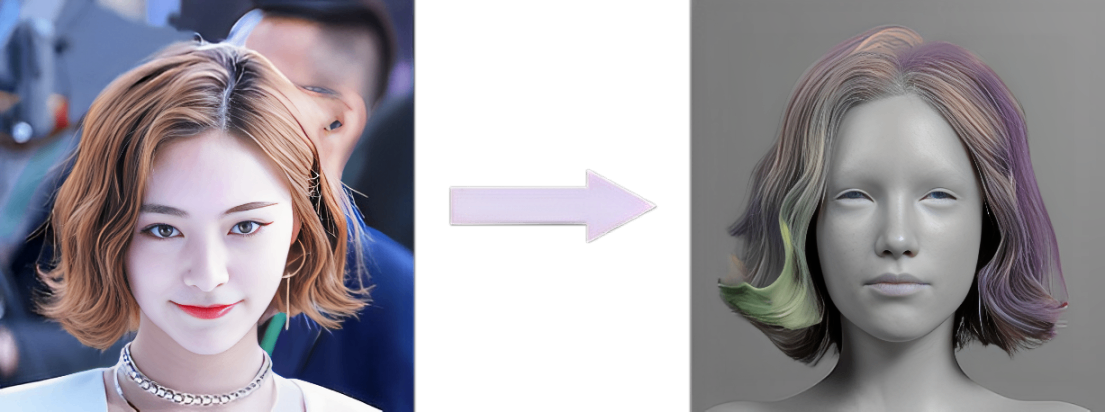
\includegraphics[width=0.8\linewidth]{assets/figures/task-intro.png}
        \caption{Single-view 3D Hair Modeling}
        \label{fig:task-intro}
    \end{figure}
\end{frame}
\newSection{Related Works}

\subsection{HairNet}
\begin{frame}\frametitle{Related Works}
    \framesubtitle{HairNet}

    \normalsize{\textcolor{myBlue}{\emph{Single-View Hair Reconstruction using Convolutional Neural Networks}}}
    
    \begin{figure}[ht]
        \centering
        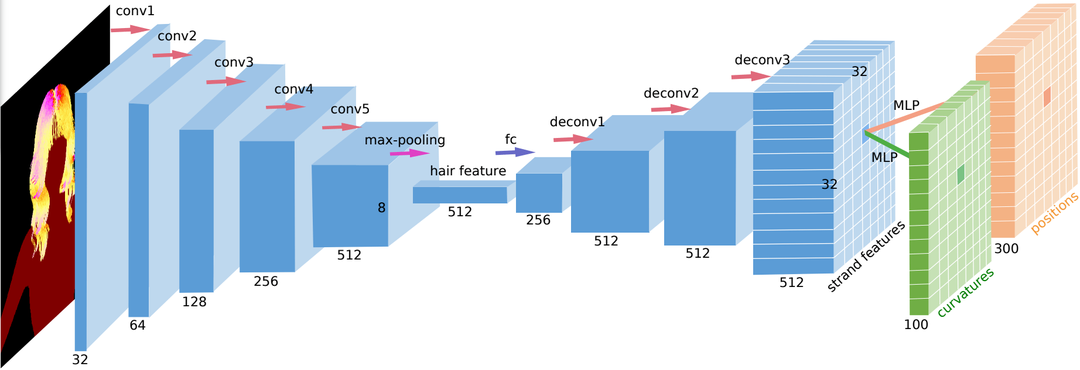
\includegraphics[width=0.8\linewidth]{assets/figures/baselines/HairNet.png}
        \caption{Zhou et al. 2018\cite{Zhou2018SingleViewHR}}
        \label{fig:hairnet}
    \end{figure}
\end{frame}


\subsection{3D Hair Synthesis}
\begin{frame}\frametitle{Related Works}
    \framesubtitle{3D Hair Synthesis}

    \normalsize{\textcolor{myBlue}{\emph{3D Hair Synthesis using Volumetric Variational Autoencoders}}}
    
    \begin{figure}[ht]
        \centering
        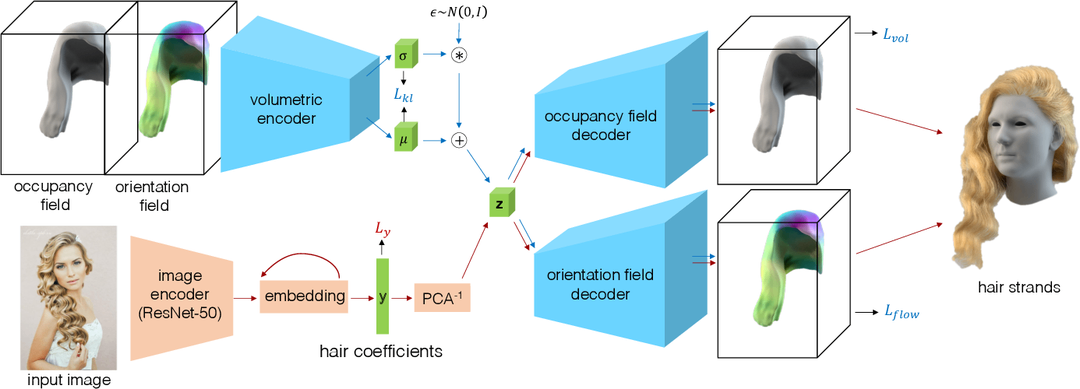
\includegraphics[width=0.8\linewidth]{assets/figures/baselines/3DHairSynthesis.png}
        \caption{Saito et al. 2018\cite{Saito20183DHS}}
        \label{fig:3dhairsynthesis}
    \end{figure}
\end{frame}


\subsection{NeuralHDHair}
\begin{frame}\frametitle{Related Works}
    \framesubtitle{NeuralHDHair}

    \normalsize{\textcolor{myBlue}{\emph{NeuralHDHair: Automatic High-fidelity Hair Modeling from a Single Image Using Implicit Neural Representations}}}
    
    \begin{figure}[ht]
        \centering
        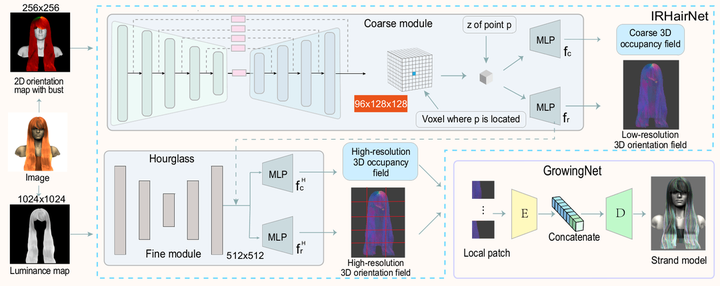
\includegraphics[width=0.8\linewidth]{assets/figures/baselines/NeuralHDHair.png}
        \caption{Wu et al. 2022\cite{wu2022neuralhdhair}}
        \label{fig:neuralhdhair}
    \end{figure}
\end{frame}


\newSection{Motivation}

%---------------------------------------------------------
\begin{frame}[t]{Motivation}
    \textbf{Main Challenge:} Using synthetic data as a prior for real-world 3D hair modeling introduces a domain gap.

    \vspace{1em}
    \textbf{Existing Solutions:} 
    \begin{itemize}
        \item Utilize undirected 2D orientation maps as an intermediate representation between the input image and the 3D hair model.
    \end{itemize}

    \vspace{1em}
    \textbf{Limitations:}
    \begin{itemize}
        \item Ambiguous directionality: Loses 3D cues from the image.
        \item Reliance on image filters: Adds noise and inaccuracies.
    \end{itemize}
\end{frame}

%---------------------------------------------------------
\begin{frame}{Undirected Orientation Maps Challenges}
    \begin{figure}
        \centering
        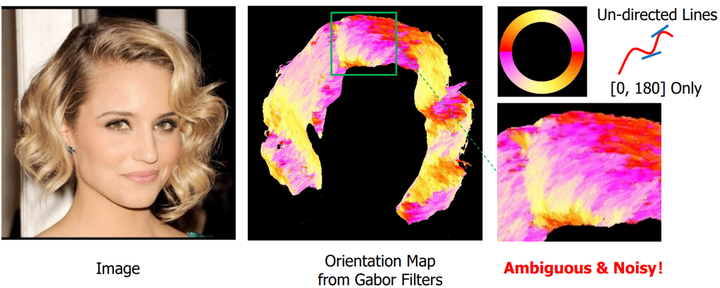
\includegraphics[width=0.9\linewidth]{assets/figures/motivations/orientation-map.png}
        \caption{Example of a 2D orientation map used in existing solutions.}
        \label{fig:motivation-orientation-map}
    \end{figure}
\end{frame}

\newSection{Contribution}

\begin{frame}[t]{Contribution}
    \begin{itemize}
        \item Proposed \emph{HairStep}, a novel intermediate representation combining strand maps and depth maps for 3D hair reconstruction.
        \item Developed a weakly-supervised domain adaptation method for depth estimation using synthetic priors and real-world sparse annotations.
        \item Created \emph{HiSa} (strand annotations) and \emph{HiDa} (relative depth annotations) datasets for 1,250 real portrait images.
        \item Introduced new metrics, \emph{HairSale} (strand alignment error) and \emph{HairRida} (relative depth accuracy), for quantitative evaluation of 3D hair modeling.
        \item Achieved state-of-the-art performance in single-view 3D hair modeling.
    \end{itemize}
\end{frame}
\newSection{Proposed Method}

%---------------------------------------------------------
\subsection{HairStep Representation}
%---------------------------------------------------------
\begin{frame}[t]{HairStep Representation}
    \emph{HairStep} is defined as $\mathbf{H} = \{\mathbf{O}, \mathbf{D}\}$ for each input image $\mathbf{I} \in \mathbb{R}^{W \times H \times 3}$, where:
    \begin{itemize}
        \item $\mathbf{O} \in \mathbb{R}^{W \times H \times 3}$ is the \textbf{Strand Map}.
        \item $\mathbf{D} \in \mathbb{R}^{W \times H \times 1}$ is the \textbf{Depth Map}.
    \end{itemize}

    \vspace{2pt}

    The \textbf{Strand Map} $\mathbf{O} \in \mathbb{R}^{W \times H \times 3}$ is defined at each pixel $x$ as:
    \begin{equation}
        \mathbf{O}(x) = \bigl(\mathbf{M}(x),\; \tfrac{\mathbf{O}_{\mathrm{2D}}(x)}{2} + 0.5\bigr),
        \label{eq:strand_map}
    \end{equation}
    \vspace{-0.5cm}
    \begin{itemize}
        \item $\mathbf{M}(x) \in \{0, 1\}$ is the hair mask indicating hair regions ($1$) and background ($0$).
        \item $\mathbf{O}_{\mathrm{2D}}(x) \in \mathbb{R}^2$ is the unit vector of 2D hair-growth orientation at pixel $x$.
    \end{itemize}

    \vspace{2pt}

    The \textbf{Depth Map} $\mathbf{D} \in \mathbb{R}^{W \times H \times 1}$ defines relative depth differences among hair strands.

    \vspace{5pt}
    \begin{itemize}
        \item Each pixel $\mathbf{D}(x) \in [0, 1]$:
        \begin{itemize}
            \item $\mathbf{D}(x) = 0$: Farthest from the camera (background or distant strands).
            \item $\mathbf{D}(x) = 1$: Closest to the camera.
        \end{itemize}
    \end{itemize}
\end{frame}

%---------------------------------------------------------
\subsection{Method Overview}
%---------------------------------------------------------
\begin{frame}[t]{Method Overview}
    The pipeline consists of three main components:
    \begin{enumerate}
        \item \textbf{Strand Map Extraction and Prediction}
        \begin{itemize}
            \item Extract strand maps from real images using the \emph{HiSa} dataset.
            \item Train a network to predict strand maps from input images.
        \end{itemize}

        \item \textbf{Domain-Adaptive Depth Estimation}
        \begin{itemize}
            \item Estimate relative depth from real images using the \emph{HiDa} dataset.
            \item Employ domain adaptation techniques to refine depth estimation.
        \end{itemize}

        \item \textbf{3D Hair Reconstruction}
        \begin{itemize}
            \item Reconstruct 3D hair strands from the predicted strand and depth maps.
            \item Utilize implicit fields for volumetric hair representation.
        \end{itemize}
    \end{enumerate}
\end{frame}

\newSection{Conclusion}

\begin{frame}[t]
    \frametitle{Conclusion}
    \textbf{Contributions:}
    \begin{itemize}
        \item Proposed \emph{HairStep}, a novel intermediate representation combining strand and depth maps.
        \item Collected new datasets \emph{HiSa} and \emph{HiDa} with annotated real images.
        \item Proposed two quantitative metrics: \emph{HairSale} and \emph{HairRida}.
        \item Achieved state-of-the-art performance in single-view 3D hair modeling.
    \end{itemize}
    \vspace{1em}
    \textbf{Limitations:}
    \begin{itemize}
        \item Manual annotation is time-consuming, limiting scalability.
        \item Generalization to unseen hairstyles and diverse real-world conditions needs further investigation.
    \end{itemize}
\end{frame}


% References
\begin{frame}[allowframebreaks, t]{References}
    \nocite{*}
    \small
    \printbibliography
\end{frame}

\end{document}
